\documentclass[journal,12pt,twocolumn]{IEEEtran}
\usepackage{cite}
\usepackage{amsmath,amssymb,amsfonts,amsthm}
\usepackage{algorithmic}
\usepackage{graphicx}
\usepackage{textcomp}
\usepackage{xcolor}
\usepackage{txfonts}
\usepackage{listings}
\usepackage{enumitem}
\usepackage{mathtools}
\usepackage{float}
\usepackage{gensymb}
\usepackage{comment}
\usepackage[breaklinks=true]{hyperref}
\usepackage{tkz-euclide} 
\usepackage{listings}
\usepackage{gvv}                                        
\def\inputGnumericTable{}                                 
\usepackage[latin1]{inputenc}                                
\usepackage{color}                                            
\usepackage{array}                                            
\usepackage{longtable}                                       
\usepackage{calc}                                             
\usepackage{multirow}                                         
\usepackage{hhline}                                           
\usepackage{ifthen}                                           
\usepackage{lscape}
\usepackage{amsmath}
\usepackage{braket}
\newtheorem{theorem}{Theorem}[section]
\newtheorem{problem}{Problem}
\newtheorem{proposition}{Proposition}[section]
\newtheorem{lemma}{Lemma}[section]
\newtheorem{corollary}[theorem]{Corollary}
\newtheorem{example}{Example}[section]
\newtheorem{definition}[problem]{Definition}
\newcommand{\BEQA}{\begin{eqnarray}}
\newcommand{\EEQA}{\end{eqnarray}}
\newcommand{\define}{\stackrel{\triangle}{=}}
\theoremstyle{remark}
\newtheorem{rem}{Remark}

\begin{document}

\bibliographystyle{IEEEtran}

\title{NCERT Discrete - 11.9.5.21}
\author{EE23BTECH11045 - Palavelli Srija$^{*}$}

\maketitle

\newpage
\bigskip

\renewcommand{\thefigure}{\theenumi}
\renewcommand{\thetable}{\theenumi}

\vspace{3cm}
\textbf{Question 11.9.5.21:} 
\begin{enumerate}
  \item Find the sum of the following series up to $n$ terms:
  \begin{enumerate}
    \item $5 + 55 + 555 + \ldots$
    \item $.6 + .66 + .666 + \ldots$
  \end{enumerate}
\end{enumerate}

\textbf{Solution:}
\begin{table}[h!]
    \centering
    \begin{table}[ht]
    \centering
    \begin{tabular}{|c|c|c|}
        \hline
        Parameter & Value & Description \\
        \hline
        $x(0)$ & 5 & First term of AP \\
        $d$ & 1.75 & Common difference of AP \\
        $x(n)$ & 20.75 & $n^{th}$ term of AP \\
        \hline
    \end{tabular}
    \vspace{2mm}
    \caption{Parameter List}
    \label{tab:simple.10.5.2.20}
\end{table}

    \caption{\textbf{Input Parameters}}
    \label{tab: table_sr5}
\end{table} 
\begin{enumerate}
\item For $x_1(n)$ :
\begin{align}
x_1(n) &= 5\brak{\frac{10^{n+1}-1}{10-1}}u(n)\\
x_1(n) & \xleftrightarrow{\mathcal{Z}} X_1(z)\\
X_1(z) &= \frac{50}{9}\brak{\frac{1}{1-10z^{-1}}}-\frac{5}{9}\brak{\frac{1}{1-z^{-1}}}, \lvert z \rvert > 10\\
s_1(n) &= 5  \sum_{i=0}^{n-1} \frac{(10^{i+1} -1)}{10-1}\\
s_1(n) &= \brak{5\frac{(10^{n+1}-1)}{10-1}}*u(n)\\
s_1(n) & \xleftrightarrow{\mathcal{Z}} S_1(z)\\
S_1(z) &= \brak{\frac{50}{9}\frac{1}{(1-10z^{-1})}-\frac{5}{9}\frac{1}{(1-z^{-1})}}\brak{\frac{1}{1-z^{-1}}} ,\lvert z \rvert > 10\\
       &=\frac{50}{81}\brak{\frac{10}{1-10z^{-1}}-\frac{1}{1-z^{-1}}}-\frac{5}{9}\brak{\frac{1}{(1-z^{-1})^2}} ,\lvert z \rvert > 10
\end{align}

from \eqref{B.9.5}
\begin{align}
s_1(n) &=\frac{50}{81}(10^{n+1}-1)u(n)-\frac{5}{9}(n+1)u(n)\\
       &=\frac{5}{81}(10^{n+2}-9n-19)u(n)  & \cbrak{n\geq0}
\end{align}
\item For $x_2(n)$ :
\begin{align}
x_2(n) &= 0.6 \brak{\frac{1-10^{-(n+1)}}{1-0.1}}u(n)\\
x_2(n) & \xleftrightarrow{\mathcal{Z}} X_2(z)\\
X_2(z) &= \frac{2}{3}\brak{\frac{1}{1-z^{-1}}}-\frac{1}{15}\brak{\frac{1}{1-(10z)^{-1}}} ,\lvert z \rvert > 1 \\
s_2(n) &= 0.6 \sum_{i=0}^{n-1} \frac{(1-10^{-(i+1)})}{1-10^{-1}}\\
s_2(n) &= \brak{0.6 \frac{(1-10^{-(n+1)})}{1-0.1}}*u(n)\\
s_2(n) & \xleftrightarrow{\mathcal{Z}} S_2(z)\\
S_2(z) &= \brak{\frac{2}{3}\frac{1}{(1-z^{-1})}-\frac{1}{15}\frac{1}{(1-(10z)^{-1})}}\brak{\frac{1}{1-z^{-1}}}, \lvert z \rvert > 1\\
   &=\frac{2}{3}\brak{\frac{1}{(1-z^{-1})^2}}\notag\\
   &-\frac{2}{27}\brak{\frac{1}{1-z^{-1}}-\frac{10^{-1}}{1-(10z)^{-1}}},\lvert z \rvert > 1
 \end{align}
   from \eqref{B.9.5}
\begin{align}
s_2(n) &=\frac{2}{3}(n+1)u(n)-\frac{2}{27}(1-10^{-(n+1)})u(n)\\
       &= \frac{2}{27}(10^{-(n+1)}+9n+8)u(n)  & \cbrak{n\geq0}
\end{align}
\end{enumerate}

\begin{figure}[h!]
    \centering
    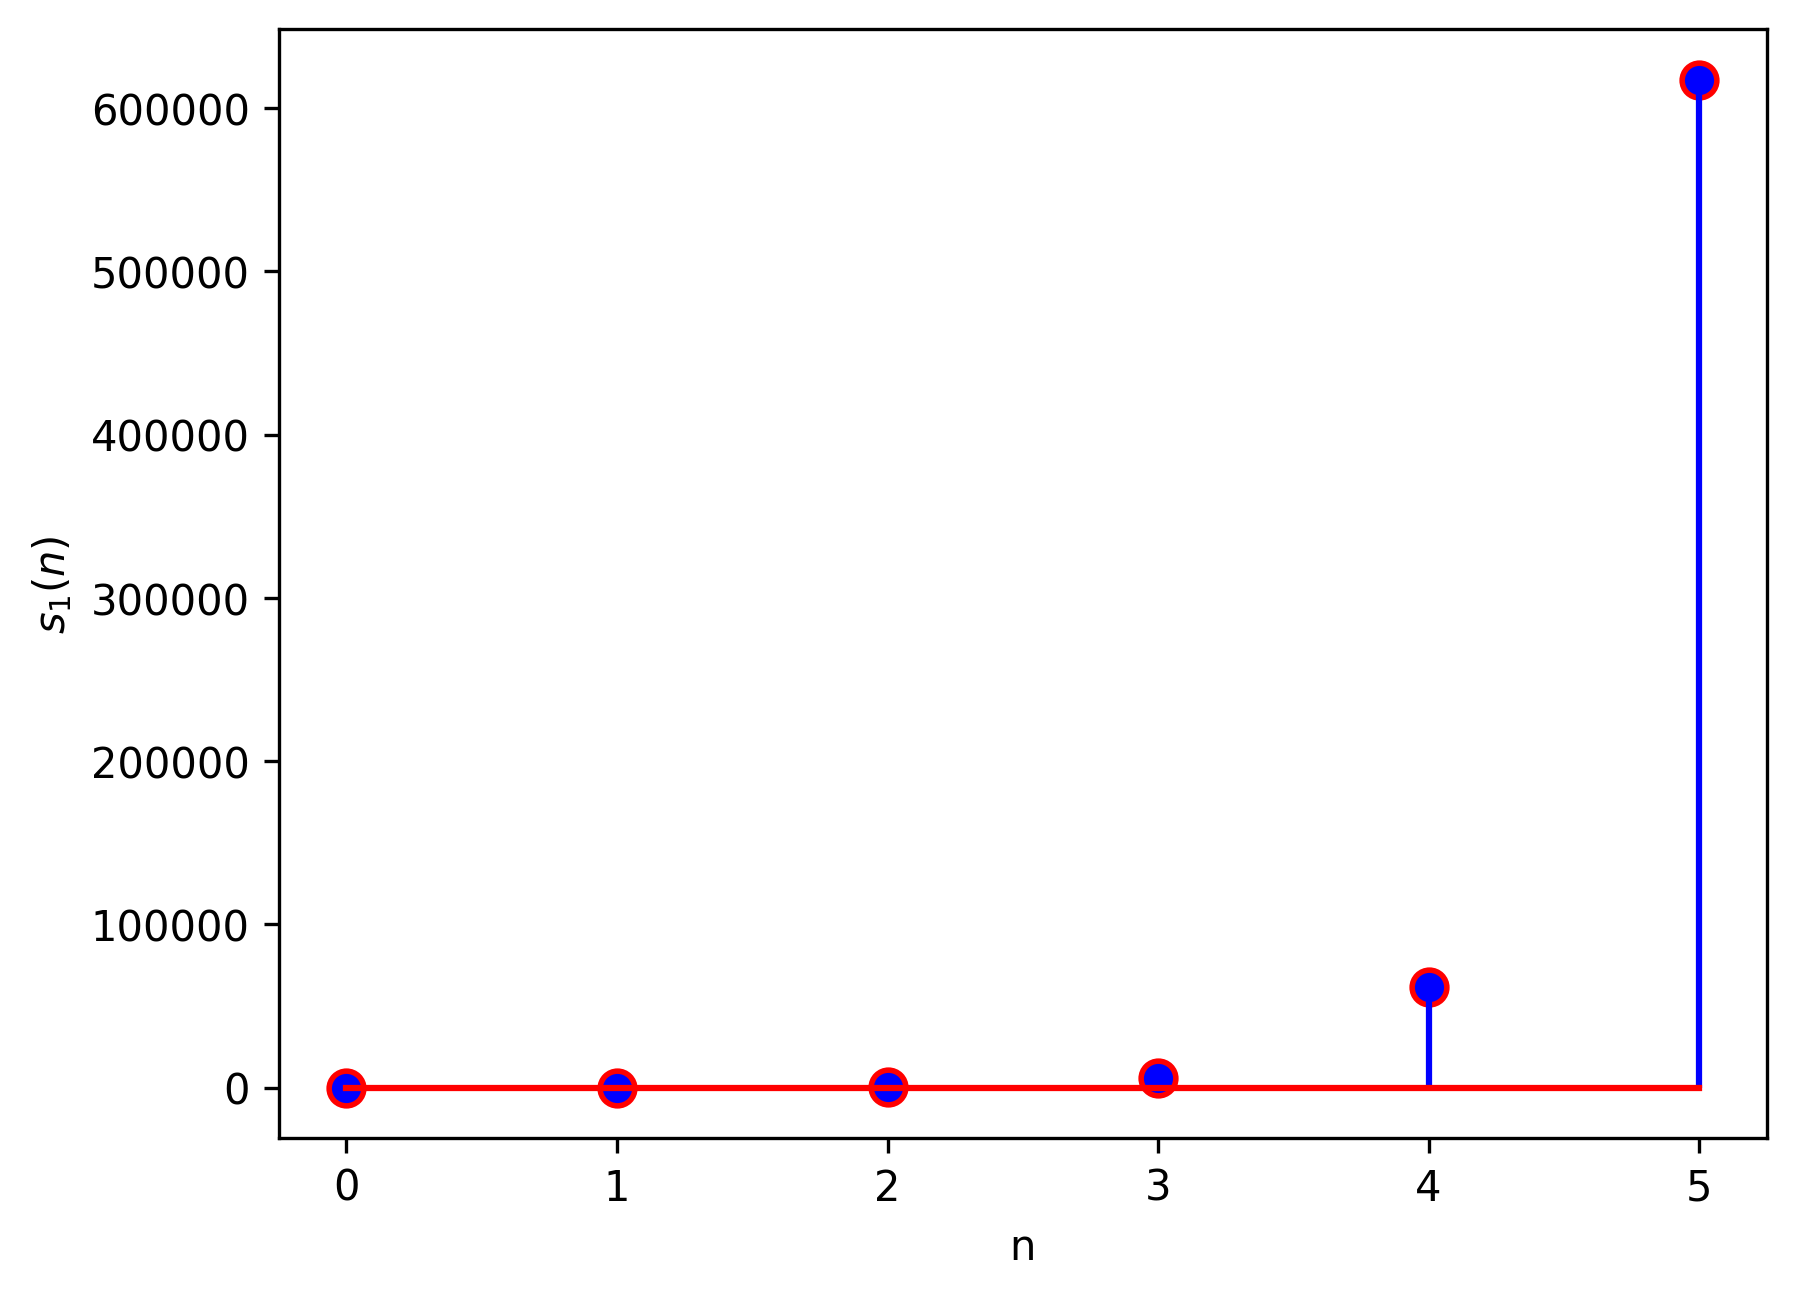
\includegraphics[width=\columnwidth]{figs/data_x1.png}
    \caption{Stem plot of $s_1(n)$}
    \label{fig: sr4}
\end{figure}
\begin{figure}[h!]
    \centering
    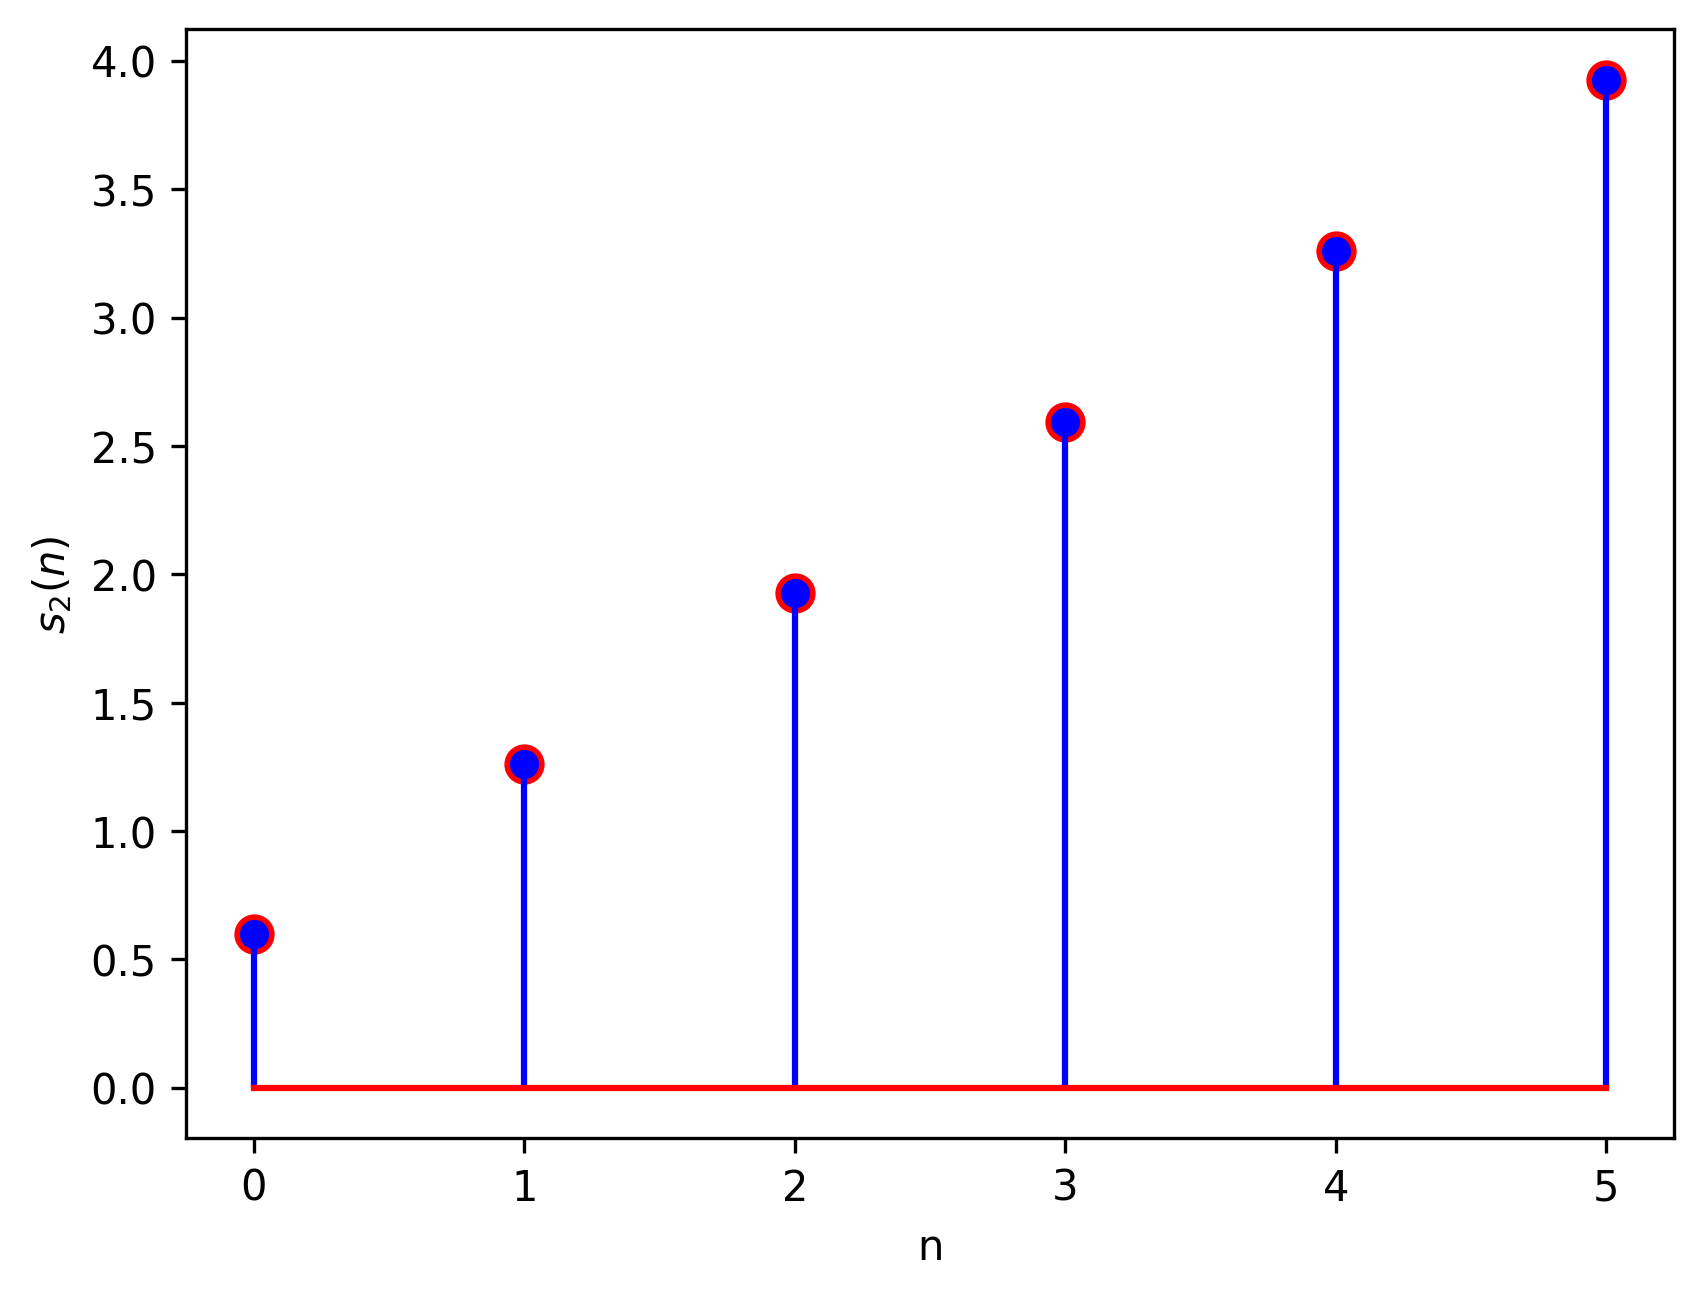
\includegraphics[width=\columnwidth]{figs/data_x2.png}
    \caption{Stem plot of $s_2(n)$}
    \label{fig: sr7}
\end{figure}

\end{document}

